\documentclass{beamer}

\mode<presentation>
{
    \usetheme{Boadilla}
  %\usetheme{default}      % or try Darmstadt, Madrid, Warsaw, ...
  \usecolortheme{default} % or try albatross, beaver, crane, ...
  \usefonttheme{default}  % or try serif, structurebold, ...
  \setbeamertemplate{navigation symbols}{}
  \setbeamertemplate{caption}[numbered]
} 

\usepackage[english]{babel}
\usepackage[utf8]{inputenc}
\usepackage[backend=bibtex,style=numeric-comp,sorting=none]{biblatex}
\addbibresource{../redaction/biblio.bib}
\usepackage{subfigure}
\usepackage{amsmath}

\usepackage{tikz,overpic}
\usetikzlibrary{fit,shapes.misc}

%\setbeamertemplate{headline}{\scriptsize{\vspace*{0.3cm}\hspace*{0.3cm}\insertframenumber}}

\title[emodiderot]{Émotions dans la musique :\\approche basée sur le contenu}
\author{Massinissa Hamidi, Hassane Gaci, Van Luan Nguyen}
\institute{Université Paris Diderot - Paris 7}
\date{07 Décembre 2016}

\begin{document}

\begin{frame} %% slide 1
 \titlepage
\end{frame} %%

%%%%%%%%%%%%%%%%%%%%%%%%%%%%%%%%%%%%%%%%%%
\begin{frame}{Motivations}
    \begin{itemize}
        \item La musique est un énorme vecteur d'émotions
        \item Curiosité, explorer d'autres types de recommandation moins
            conventionnels
        \item interêt grandissant pour les émotions de la part des acteurs du
            domaine du Music Information Retrieval (MIR)
    \end{itemize}
\end{frame}

%%%%%%%%%%%%%%%%%%%%%%%%%%%%%%%%%%%%%%%%%%
\section{Reconnaissance des émotions}

\begin{frame}{Plan}
      \tableofcontents[currentsection]
  \end{frame}

\begin{frame}{Paradigmes de représentation des émotions}
\begin{figure}
\centering
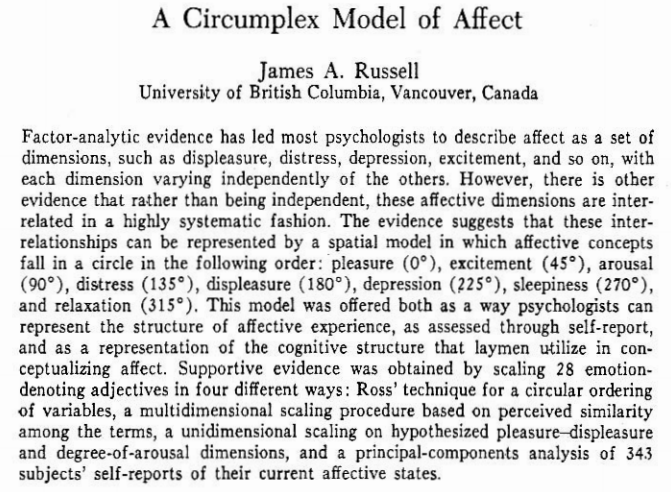
\includegraphics[width=200px]{images/a_circumplex_model_of_affect.png}
\footfullcite{citeulike:630522}
\end{figure}
\end{frame}
%%%%%%%%%%%%%%%%%%%%%%%%%%%%%%%%%%%%%%%%%%
\begin{frame}{Modèle de Russell (psychologie)}
\begin{itemize}
    \item En psychologie, le terme valence est utilisé pour désigner la qualité
        intrinsèquement agréable ou désagréable d'un stimulus ou d'une
        situation (axe horizontal).

    \item le terme activation représente le niveau d'excitation corporelle qui
        correspond dans notre cas au rythme musical (axe vertical)
\end{itemize}

\end{frame}

\begin{frame}{Modèle de Russell (psychologie)}


        \begin{figure}
            \centering
            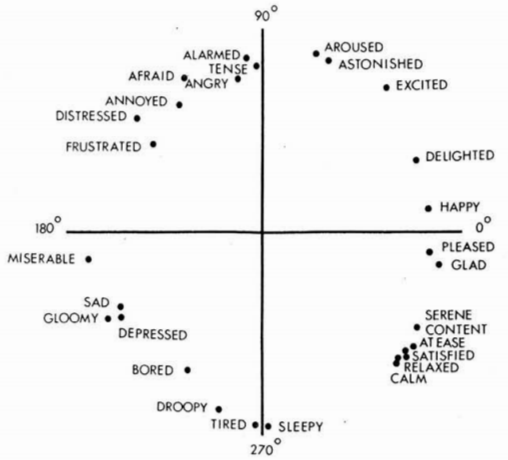
\includegraphics[width=200px]{images/russell_2.png}
            \footfullcite{citeulike:630522}
        \end{figure}

\end{frame}

%%%%%%%%%%%%%%%%%%%%%%%%%%%%%%%%%%%%%%%%%%%
\section{Données}
\begin{frame}{Plan}
      \tableofcontents[currentsection]
  \end{frame}

\begin{frame}{The Million Song Dataset}
\begin{figure}
\centering
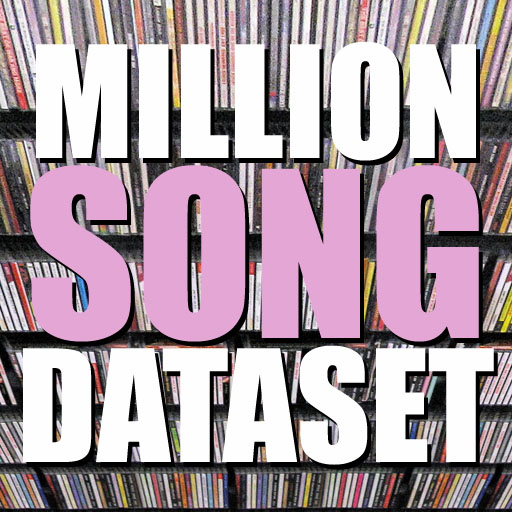
\includegraphics[width=140px]{images/millionsong2.jpg}
\end{figure}
\footfullcite{Bertin-Mahieux2011}
% il a été crée suite à une colaboration entre le labrosa et echonest.
% en effet un certain nombre de features ont été obtenues à partir de l'api
% echonest, parmi celle-ci, tempo, loudness, timings of fade-in and fade-out,
% and MFCC-like features
%
% les buts de cette initiative:
%  - To encourage research on algorithms that scale to commercial sizes
%  - To provide a reference dataset for evaluating research
%  - As a shortcut alternative to creating a large dataset with APIs (e.g. The EchoNest's)
%  - To help new researchers get started in the MIR field
%
% Limitations:
% Diversity is another issue: there is little or no world, ethnic,
% and classical music
\end{frame}

%%%%%%%%%%%%%%%%%%%%%%%%%%%%%%%%%%%%%%%%%%
\begin{frame}{Million Song Dataset Benchmarks}
    \begin{itemize}
        \item En utilisant un content provider, 7digital en l'occurrence, les
            chercheurs de l'université de vienne ont pu avoir accèes à des
            extraits des chansons répertoriées dans MSD
            \footfullcite{schindler2012facilitating}
        \item Calcule de nouvelles caractéristiques à l'aide des outils
            \texttt{jAudio} et \texttt{Marsyas}
        \item Nous n'avons toujours pas les tags relatifs aux émotions
    \end{itemize}
%The dataset does however not provide an easy download possibility for the
%audio files, thus researchers are basically limited to the features provided
%with the dataset. Using a content provider, for which links with unique IDs to
%the internal database existed in the MSD, we downloaded audio samples, mostly
%in the form of 30 or 60 second snippets. Subsequently, we provide a multitude
%of features extracted from these samples, to allow comparison between them.

\end{frame}

%%%%%%%%%%%%%%%%%%%%%%%%%%%%%%%%%%%%%%%%%%
%\begin{frame}{Caractéristiques extraites à partir du MSD}
%    \begin{figure}
%        \centering
%        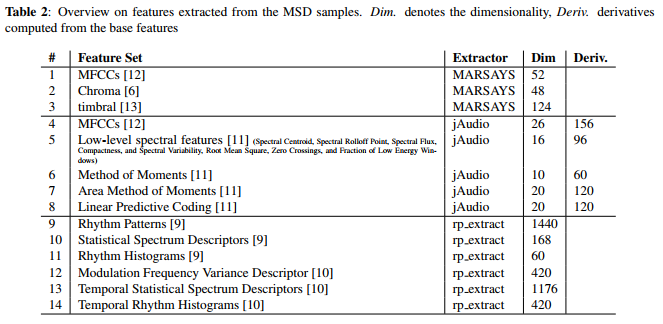
\includegraphics[width=150px]{images/overview_on_features_extracted_from_msd.png}
%        \footfullcite{Bertin-Mahieux2011}
%    \end{figure}
%    jAudio: Software for extracting low and high-level features from audio
%    recordings.
%    Marsyas (Music Analysis, Retrieval and Synthesis for Audio Signals) is an
%    open source software framework for audio processing with specific emphasis
%    on Music Information Retrieval applications
%\end{frame}

%%%%%%%%%%%%%%%%%%%%%%%%%%%%%%%%%%%%%%%%%%
\begin{frame}{Annotations lastfm} %% slide 4
\begin{figure}
\centering

\includegraphics[width=150px]{images/lastfm.jpg}
\end{figure}
\begin{itemize}
    \item Réseau social de plus de 30 millions d'utilisateurs
    \item Écouter, annoter des musiques
    \item Donne accès aux annotations des utilisateurs entre autres,
        via une api
    \item 505,216 tracks avec au moins un tag
    \item 522,366 tags uniques
\end{itemize}
%\begin{itemize}
%    \item c'est quoi déja?
%        The Last.fm dataset is similar to the beaTunes database,
%        in that it also contains multiple user-submitted labels per
%        song which are each associated with a weight.
%    \item qui a fait les annotations?
%    \item ont elles été vérifiées?
%    \item quelle valeur peut on donner à ces annotations?
%    \item ont elles déja été utilisées dans des études?
%    \item comment est-ce fait?
%    \item quelles mots clés ont été selectionnés et comment?
%\end{itemize}
\end{frame} %%
%%%%%%%%%%%%%%%%%%%%%%%%%%%%%%%%%%%%%%%%%%

%%%%%%%%%%%%%%%%%%%%%%%%%%%%%%%%%%%%%%%%%%
\section{Méthodes et traitements}

\begin{frame}{Plan}
    \tableofcontents[currentsection]
\end{frame}


\begin{frame}{Représentation spaciale des tags}
    \begin{itemize}
        \item À partir des annotations des utilisateurs d'un réseau sociale
            musical tel que lastfm, inférer une représentation spaciale des
            tags relatifs aux
            émotions~\footfullcite{laurier2011automatic}~\footfullcite{saari2014semantic}
    \end{itemize}
\begin{figure}
    \begin{subfigure}
    \centering
    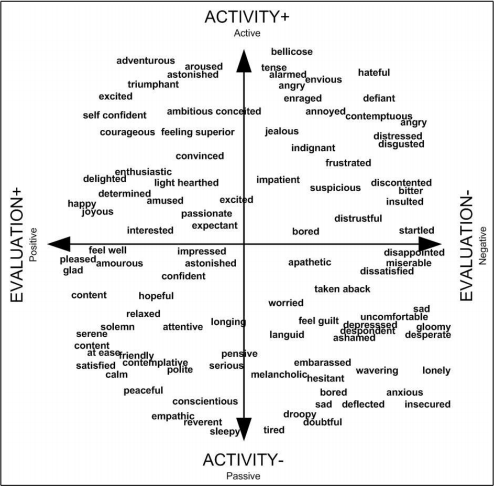
\includegraphics[width=120px]{images/scherer_model.png}
    \end{subfigure}
    \hspace{12px}
    \begin{subfigure}
    \centering
    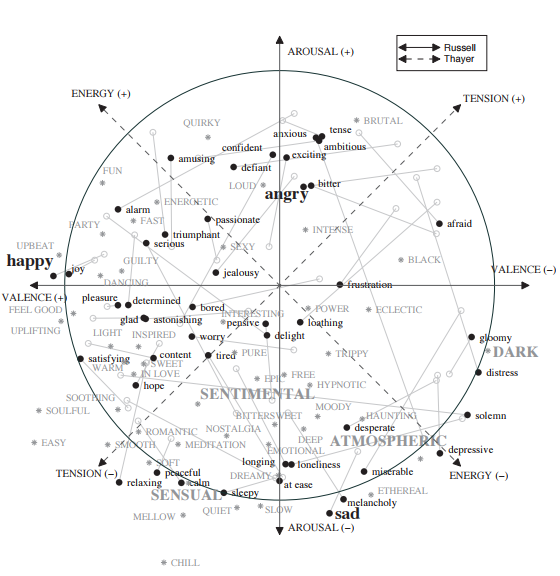
\includegraphics[width=120px]{images/result_mood_space.png}
    \end{subfigure}

\end{figure}
\end{frame}
%%%%%%%%%%%%%%%%%%%%%%%%%%%%%%%%%%%%%%%%%%

\begin{frame}{Term-Document Matrix}
    \begin{itemize}
        \item Les tags en colonnes et les chansons en lignes
        \item Pour chaque chanson, les tf-idf des tags qui lui correspondent
        \item Résulte en une matrice creuse
    \end{itemize}

    \[
        \textrm{ tags}
        \stackrel{\mbox{chansons}}{
    \begin{bmatrix}
            x_{11} & x_{12} & x_{13} & \dots  & x_{1n} \\
            x_{21} & x_{22} & x_{23} & \dots  & x_{2n} \\
            \vdots & \vdots & \vdots & \ddots & \vdots \\
            x_{d1} & x_{d2} & x_{d3} & \dots  & x_{dn}
    \end{bmatrix}
}
\]

\end{frame}

%%%%%%%%%%%%%%%%%%%%%%%%%%%%%%%%%%%%%%%%%%

\begin{frame}{LSA \& SVD}
\begin{figure}
    \centering
    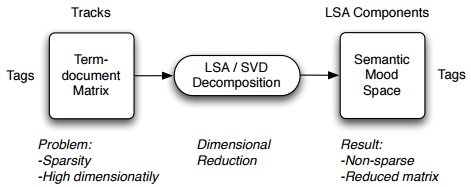
\includegraphics[width=200px]{images/lsa_cyril_laurier.png}
    \footfullcite{laurier2011automatic}
\end{figure}
\begin{itemize}
    \item Choix d'un rang $k$ pour l'approximation
    \item La réduction de dimensionalité doit permettre de fusionner les
        dimensions associées à des tags qui ont la même signification.
\end{itemize}

\end{frame}
%%%%%%%%%%%%%%%%%%%%%%%%%%%%%%%%%%%%%%%%%%
\begin{frame}{Distances entre termes}
    \begin{itemize}
        \item $d_{cos}(scary, fun) = 0.99$
        \item $d_{cos}(tense, serene) = 0.98$
        \item $d_{cos}(anger, aggressive) = 0.06$
        \item $d_{cos}(calm, relaxed) = 0.03$
    \end{itemize}
\end{frame}

%%%%%%%%%%%%%%%%%%%%%%%%%%%%%%%%%%%%%%%%%%
\begin{frame}{Et maintenant!}
\begin{figure}
    \centering
    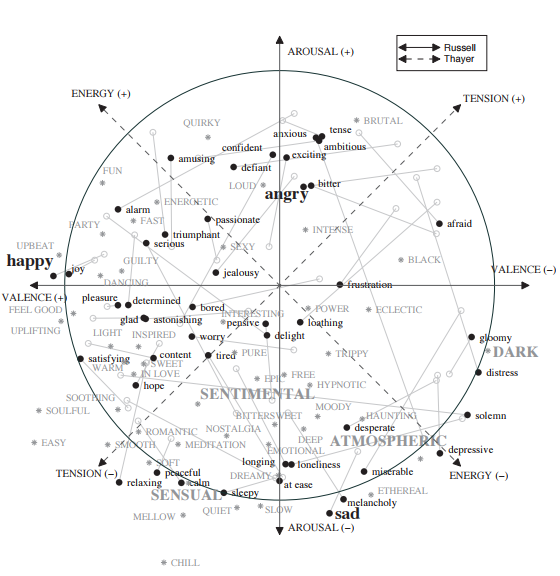
\includegraphics[width=220px]{images/result_mood_space.png}
\end{figure}

\end{frame}

%%%%%%%%%%%%%%%%%%%%%%%%%%%%%%%%%%%%%%%%%%
\begin{frame}{Croisement avec les données de tuwien}
    \begin{figure}
        \centering
        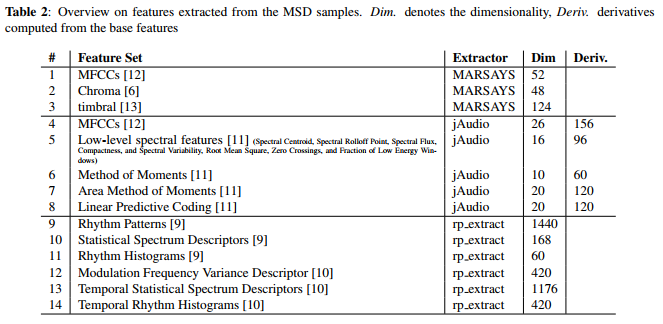
\includegraphics[width=250px]{images/overview_on_features_extracted_from_msd.png}
        \footfullcite{schindler2012facilitating}
    \end{figure}
\end{frame}

%%%%%%%%%%%%%%%%%%%%%%%%%%%%%%%%%%%%%%%%%%
\begin{frame}{Problème de régression}
    au final, la prédiction se résume en la détérmination, pour une chanson
    donnée et un set de caractéristiques de bas et de haut niveau calculées
    sur celle-ci, d'un point dans l'espace des émotions obtenu auparavent.
\end{frame}

%\begin{frame}{Ce sur quoi j'ai travaillé}
%\only<1>{
%\centering
%\begin{overpic}[width=200px]{images/step.png}
%
%\end{overpic}}%
%
%\only<2>{
%\centering
%\begin{overpic}[width=200px]{images/step.png}
%\put(-1,0){\tikz \draw[red,thick,rounded corners] (0,0) rectangle (1.75,1.5);}
%\end{overpic}}%
%
%\only<3>{
%\centering
%\begin{overpic}[width=200px]{images/step.png}
%\put(25.5,0){\tikz \draw[red,thick,rounded corners] (0,0) rectangle (1.75,1.5);}
%\end{overpic}}%
%
%\only<4>{
%\centering
%\begin{overpic}[width=200px]{images/step.png}
%\put(25.5,0){\tikz \draw[red,thick,rounded corners] (0,0) rectangle (1.75,1.5);}
%\end{overpic}}%
%
%\only<5>{
%\centering
%\begin{overpic}[width=200px]{images/step.png}
%\put(52.5,0){\tikz \draw[red,thick,rounded corners] (0,0) rectangle (4,1.7);}
%\end{overpic}}%
%
%\begin{overprint}
%  \onslide<1> 
%
%	\onslide<2>
%    \begin{itemize}
%	\item Voice Activity Detector~\footfullcite{sohn1999statistical}.
%    \item Estimation du spectre du bruit~\footfullcite{cohen2003noise} à l'aide du Improved Minima Controlled Recursive Averaging 
%    \begin{equation}
%    \begin{aligned}
%    & H_{0} : \lambda_{n,k}(l+1) = a_{n}\lambda_{n,k}(l)+(1-a_{n})|X_{k}(l)|^{2} \\				
%    & H_{1} : \lambda_{n,k}(l+1) = \lambda_{n,k}(l)
%    \end{aligned}
%    \label{eq:mcra_hypothesis}
%    \end{equation}
%    \item  le pitch des nourrissons est compris entre 300 et 600 Hz~\footfullcite{cohen2012infant}
%	\end{itemize}
%  
%  \onslide<3>
%  \begin{itemize}%%%%%%
%  	\item Normalisation du signal % afin d'avoir des données uniforme pour les différentes transformées que l'on effectue et les fenetres qu'on applique
%  	\item End-Point Detection avec l'utilisation de la Short-Time Energy du signal et du Zero-Crossing Rate~\footfullcite{diaz2012automatic}
%  	\item Élimination des parties dont la durée est inférieure à 250ms % cette partie va nous permettre d'éliminer les portions du signal qui ne correspondent pas à une énonciation
%  	\item Application de filtres et fenêtrage
%
%\item Transformée de Fourrier
%\begin{equation}
%X = \sum_{n=0}^{N-1} x_{n}.\exp\{\frac{2\pi i k n}{N}\}
%\end{equation}
%  \end{itemize}%%%%%
%
%	\onslide<4>
%      % elles sont au nombre de 15 dans les travaux de
%  \begin{itemize}%%%%%%
%  \item Les caractéristiques sont au nombre de 15 dans les travaux de Chuan-Yu Chang~\footfullcite{chang2016dag}
%      \begin{itemize}
%      %il y a beaucoup de variantes mais elles se basent toutes sur la formule d'autocoréllation
%      \item détection du pitch
%      \begin{equation}
%		\scriptsize
%        \rho_{ff}(\tau)= \int_{0}^{T}x(t)x(t+\tau)dt
%	  \end{equation}
%      \item Zero-Crossing Rate
%      \begin{equation}
%      	\scriptsize
%      	ZCR = \sum_{n=1}^{N-1}|sgn(x_{n}-sgn(x_{n-1}))|
%	  \end{equation}
%      \item spectral centroid ...
%      %\item ...
%      \end{itemize}
%  \end{itemize}%%%%%
%  
%	\onslide<5>
%  	\begin{itemize}
%  	\item Machine à Vecteurs de support, régression linéaire, arbres de décision, ... 
%    \vspace{3px}
%    \begin{figure}
%	\centering
%    \includegraphics[width=200px]{images/oneVsAllClassification.png}
%	\end{figure}
%	\end{itemize}
%
%\end{overprint}
%\end{frame}
%
%\begin{frame}{Conclusions}
%\centering
%\begin{itemize}
%\item apports techniques
%\item apports au niveau personnel
%\item perspectives
%\end{itemize}
%
%\end{frame}
%%%%%%%%%%%%%%%%%%%%%%%%%%%%%%%%%%%%%%%%%%%
%
%\begin{frame}
%\centering
%\LARGE Demo
%\end{frame}

%%%%%%%%%%%%%%%%%%%%%%%%%%%%%%%%%%%%%%%%%%
\begin{frame}
\centering
\LARGE Questions
\end{frame}
\end{document}
